\documentclass{sig-alternate-ipsn13}
\usepackage{ntheorem}
\usepackage{algorithm}
\usepackage[noend]{algorithmic}
\usepackage{todonotes}
\usepackage{enumitem}


%-----------------------------------------------------------------------------------------------------------------------------------------------------------------
% Sets
\newcommand{\Fbb}{\mathbb{F}}
\newcommand{\Rbb}{\mathbb{R}}
\newcommand{\Cbb}{\mathbb{C}}
\newcommand{\Nbb}{\mathbb{N}}
\newcommand{\Qbb}{\mathbb{Q}}
\newcommand{\Zbb}{\mathbb{Z}}

\newcommand{\Acal}{\mathcal{A}}
\newcommand{\Bcal}{\mathcal{B}}
\newcommand{\Ccal}{\mathcal{C}}
\newcommand{\Dcal}{\mathcal{D}}
\newcommand{\Ecal}{\mathcal{E}}
\newcommand{\Fcal}{\mathcal{F}}
\newcommand{\Gcal}{\mathcal{G}}
\newcommand{\Hcal}{\mathcal{H}}
\newcommand{\Ical}{\mathcal{I}}
\newcommand{\Jcal}{\mathcal{J}}
\newcommand{\Kcal}{\mathcal{K}}
\newcommand{\Lcal}{\mathcal{L}}
\newcommand{\Mcal}{\mathcal{M}}
\newcommand{\Ncal}{\mathcal{N}}
\newcommand{\Ocal}{\mathcal{O}}
\newcommand{\Pcal}{\mathcal{P}}
\newcommand{\Qcal}{\mathcal{Q}}
\newcommand{\Rcal}{\mathcal{R}}
\newcommand{\Scal}{\mathcal{S}}
\newcommand{\Tcal}{\mathcal{T}}
\newcommand{\Ucal}{\mathcal{U}}
\newcommand{\Vcal}{\mathcal{V}}
\newcommand{\Wcal}{\mathcal{W}}
\newcommand{\Xcal}{\mathcal{X}}
\newcommand{\Ycal}{\mathcal{Y}}
\newcommand{\Zcal}{\mathcal{Z}}

\newcommand{\bigO}{\Ocal}

%-----------------------------------------------------------------------------------------------------------------------------------------------------------------
% operators
\DeclareMathOperator*{\argmax}{arg\,max}
\DeclareMathOperator*{\argmin}{arg\,min}
\DeclareMathOperator*{\cart}{\times}
\DeclareMathOperator*{\card}{card}
\DeclareMathOperator*{\superset}{\supset}
\DeclareMathOperator*{\support}{support}

% calculus
\newcommand \ddt[1]{\frac{d #1}{dt}}
\newcommand \ppx[1]{\frac{\partial #1}{\partial x}}
\newcommand \ppxn[2]{\frac{\partial^{#2} #1}{\partial^{#2} x}}
\newcommand \ddtn[2]{\frac{d^{#2} #1}{dt^{#2}}}

% topology
\DeclareMathOperator*{\bd}{bd}
\DeclareMathOperator*{\osc}{osc}
\DeclareMathOperator*{\disc}{disc}
\DeclareMathOperator*{\cl}{cl}
\DeclareMathOperator*{\interior}{int}

% linear albegra
\DeclareMathOperator*{\dm}{dim}
\DeclareMathOperator*{\spn}{span}
\DeclareMathOperator*{\trace}{trace}
\DeclareMathOperator*{\Tr}{Tr}
\DeclareMathOperator*{\diag}{diag}

% probability
\DeclareMathOperator*{\cov}{cov}
\DeclareMathOperator*{\var}{var}
\DeclareMathOperator*{\Exp}{\mathbb{E}}
\newcommand\Expsq[1]{\Exp\sqbr{#1}}
\DeclareMathOperator*{\Pro}{\mathbb{P}}
\DeclareMathOperator*{\Prob}{\mathbb{P}}
\newcommand \convL[1]{\overset{L^{#1}}{\rightarrow} }
\newcommand \convP{\overset{\text{P}}{\rightarrow} }
\newcommand \convAS{\overset{\text{a.s.}}{\rightarrow} }



%convex optimization
\DeclareMathOperator*{\Co}{Co}
\DeclareMathOperator*{\conv}{conv}
\DeclareMathOperator*{\diam}{diam}

%complex
\DeclareMathOperator*{\Real}{Re}
\DeclareMathOperator*{\Imag}{Im}
\newcommand\contains{\ni}



%-----------------------------------------------------------------------------------------------------------------------------------------------------------------
% text
\newcommand{\by}{\text{ by }}
\newcommand{\pf}{\paragraph{\emph{proof}}}
\newcommand\p[1]{\paragraph{#1}}
\newcommand{\ans}{\paragraph{\emph{answer}}}
\newcommand{\subjectto}{\text{subject to}}
\newcommand\ind[1]{1_{#1}}

\newcommand\emp[1]{{\color{Red} #1}}

%-----------------------------------------------------------------------------------------------------------------------------------------------------------------
% matrices and equations

\newcommand \func[5]{
\[
\begin{aligned}
#1: #2 &\rightarrow #3 \\
#4 &\mapsto #5
\end{aligned}
\]
}

\newcommand \al[1]{\begin{align*}
#1
\end{align*}
}

\newcommand \aln[1]{\begin{align}
#1
\end{align}
}

\newcommand \ald[1]{
\[
\begin{aligned}
#1
\end{aligned}
\]
}

\newcommand \aldn[1]{
\begin{equation}
\begin{aligned}
#1
\end{aligned}
\end{equation}
}


\newcommand \mat[1]{
\left(
\begin{array}
#1
\end{array}
\right)
}

\newcommand \Det[1]{
\left|
\begin{array}
#1
\end{array}
\right|
}
%-----------------------------------------------------------------------------------------------------------------------------------------------------------------
%other
\newcommand{\horline}{
\begin{center}
\line(1,0){500}
\end{center}
}

\newcommand \vs{\vspace{40pt}}

\newcommand \imp{\Rightarrow}
\newcommand \eqv{\Leftrightarrow}



%-----------------------------------------------------------------------------------------------------------------------------------------------------------------
% parenthesis and such
\newcommand \floor[1]{\lfloor #1 \rfloor}
\newcommand \ceil[1]{\left\lceil #1 \right\rceil}
\newcommand \bra{\left\langle}
\newcommand \ket{\right\rangle}
\newcommand \braket[2]{\bra #1, #2 \ket}
\newcommand{\psh}[2]{\ensuremath{\langle #1,#2\rangle}}
\newcommand \parenth[1]{\left( #1 \right)}
\newcommand \curl[1]{\left\{ #1 \right\}}
\newcommand \sqbr[1]{\left[ #1 \right]}
\newcommand \sqbra[1]{\left[ #1 \right]}


%-----------------------------------------------------------------------------------------------------------------------------------------------------------------







%-----------------------------------------------------------------------------------------------------------------------------------------------------------------
% Algorithms
\usepackage{listings} % for algorithms
\usepackage{framed}
% setup of the lst
\lstset{ %
  basicstyle=\footnotesize,
  commentstyle=\color{gray},
  extendedchars=true,
  frame=single,
  keywordstyle=\color{blue},
  language=Java,
  morekeywords={trait, def, val},
  numbers=left,
  numbersep=5pt,
  numberstyle=\tiny\color{gray},
  tabsize=2
}




\newtheorem{remark}{Remark}
\newtheorem{theorem}{Theorem}
\newtheorem*{nonumtheorem}{Theorem}
\newtheorem{definition}{Definition}
\newtheorem{proposition}{Proposition}


% \usepackage{picins}
% \usepackage{graphicx}

% \makeatletter
% \def\Ginclude@graphics#1{%
%   \parpic(\Gin@@ewidth,\Gin@@eheight)[d]{#1}\picskip{0}}%
% \makeatother


\begin{document}

\title{On Learning How Players Learn:\\
Estimation of Learning Dynamics in the Routing Game
% \titlenote{}
}
%
% You need the command \numberofauthors to handle the 'placement
% and alignment' of the authors beneath the title.
%
% For aesthetic reasons, we recommend 'three authors at a time'
% i.e. three 'name/affiliation blocks' be placed beneath the title.
%
% NOTE: You are NOT restricted in how many 'rows' of
% "name/affiliations" may appear. We just ask that you restrict
% the number of 'columns' to three.
%
% Because of the available 'opening page real-estate'
% we ask you to refrain from putting more than six authors
% (two rows with three columns) beneath the article title.
% More than six makes the first-page appear very cluttered indeed.
%
% Use the \alignauthor commands to handle the names
% and affiliations for an 'aesthetic maximum' of six authors.
% Add names, affiliations, addresses for
% the seventh etc. author(s) as the argument for the
% \additionalauthors command.
% These 'additional authors' will be output/set for you
% without further effort on your part as the last section in
% the body of your article BEFORE References or any Appendices.

\numberofauthors{3} %  in this sample file, there are a *total*
% of EIGHT authors. SIX appear on the 'first-page' (for formatting
% reasons) and the remaining two appear in the \additionalauthors section.
%
\author{
% You can go ahead and credit any number of authors here,
% e.g. one 'row of three' or two rows (consisting of one row of three
% and a second row of one, two or three).
%
% The command \alignauthor (no curly braces needed) should
% precede each author name, affiliation/snail-mail address and
% e-mail address. Additionally, tag each line of
% affiliation/address with \affaddr, and tag the
% e-mail address with \email.
%
% 1st. author
\alignauthor Kiet Lam\\
\affaddr{UC Berkeley}
\email{\small\texttt{kiet.lam@berkeley.edu}}
\alignauthor Walid Krichene\\
\affaddr{UC Berkeley}
\email{\small\texttt{walid@eecs.berkeley.edu}}
\alignauthor Alexandre Bayen\\
\affaddr{UC Berkeley}
\email{\small\texttt{bayen@berkeley.edu}}
% \alignauthor
% Ben Trovato\titlenote{Dr.~Trovato insisted his name be first.}\\
%        \affaddr{Institute for Clarity in Documentation}\\
%        \affaddr{1932 Wallamaloo Lane}\\
%        \affaddr{Wallamaloo, New Zealand}\\
%        \email{trovato@corporation.com}
% % 2nd. author
% \alignauthor
% G.K.M. Tobin\titlenote{The secretary disavows
% any knowledge of this author's actions.}\\
%        \affaddr{Institute for Clarity in Documentation}\\
%        \affaddr{P.O. Box 1212}\\
%        \affaddr{Dublin, Ohio 43017-6221}\\
%        \email{webmaster@marysville-ohio.com}
% % 3rd. author
% \alignauthor Lars Th{\o}rv{\"a}ld\titlenote{This author is the
% one who did all the really hard work.}\\
%        \affaddr{The Th{\o}rv{\"a}ld Group}\\
%        \affaddr{1 Th{\o}rv{\"a}ld Circle}\\
%        \affaddr{Hekla, Iceland}\\
%        \email{larst@affiliation.org}
% \and  % use '\and' if you need 'another row' of author names
% % 4th. author
% \alignauthor Lawrence P. Leipuner\\
%        \affaddr{Brookhaven Laboratories}\\
%        \affaddr{Brookhaven National Lab}\\
%        \affaddr{P.O. Box 5000}\\
%        \email{lleipuner@researchlabs.org}
% % 5th. author
% \alignauthor Sean Fogarty\\
%        \affaddr{NASA Ames Research Center}\\
%        \affaddr{Moffett Field}\\
%        \affaddr{California 94035}\\
%        \email{fogartys@amesres.org}
% % 6th. author
% \alignauthor Charles Palmer\\
%        \affaddr{Palmer Research Laboratories}\\
%        \affaddr{8600 Datapoint Drive}\\
%        \affaddr{San Antonio, Texas 78229}\\
%        \email{cpalmer@prl.com}
}
% There's nothing stopping you putting the seventh, eighth, etc.
% author on the opening page (as the 'third row') but we ask,
% for aesthetic reasons that you place these 'additional authors'
% in the \additional authors block, viz.
% \additionalauthors{Additional authors: John Smith (The Th{\o}rv{\"a}ld Group,
% email: {\texttt{jsmith@affiliation.org}}) and Julius P.~Kumquat
% (The Kumquat Consortium, email: {\texttt{jpkumquat@consortium.net}}).}
% \date{30 July 1999}
% Just remember to make sure that the TOTAL number of authors
% is the number that will appear on the first page PLUS the
% number that will appear in the \additionalauthors section.

\maketitle
\begin{abstract}
  The routing game models congestion in transportation networks, communication networks, and other cyber physical systems in which agents compete for shared resources.
  We consider an online learning model of player dynamics: at each iteration, every player chooses a route (or a probability distribution over routes, which corresponds to a flow allocation over the physical network), then the joint decision of all players determines the costs of each path, which are then revealed to the players.

  We pose the following estimation problem: given a sequence of player decisions and the corresponding costs, we would like to estimate the learning model parameters. We consider in particular entropic mirror descent dynamics, reduce the problem to estimating the learning rates of each player.

  We demonstrate this method using data collected from a routing game experiment, played by human participants: We develop a web application to implement the routing game. When players log in, they are assigned an origin and destination on the graph. They can choose, at each iteration, a distribution over their available routes, and each player seeks to minimize her own cost. We collect a data set using this interface, then apply the proposed method to estimate the learning model parameters.
  We observe in particular that after an exploration phase, the joint decision of the players remains within a small distance of the Nash equilibrium. We also use the estimated model parameters to predict the flow distribution over routes, and compare these predictions to the actual distribution.
  Finally, we discuss some of the qualitative implications of the experiments, and give directions for future research.

\end{abstract}

%============================================================================================
\section{Introduction}
The routing game is a non-cooperative game that models congestion in many cyber physical systems (CPS) in which non-cooperative agents compete for shared resources, such as transportation networks (the resources being roads) and communication networks (the resources being communication links)~\cite{beckmann1955studies,roughgarden2007,ozdaglar2007incentives}. The game is played on a directed graph that represents the network, and each player is given by a source node and destination node, and seeks to send traffic (either packets in a communication setting, or cars in a  transportation setting) while minimizing the total delay of that traffic. The delay is determined by the joint decision of all players, such that whenever an edge has high load, it becomes congested and any traffic using that edge incurs additional delay, defined by a congestion function that models the underlying physical process. This model of congestion is simple yet powerful, and routing games have been studied extensively since the seminal work of Beckman~\cite{beckmann1955studies}.

\subsection{Learning models and convergence to Nash equilibria}
The Nash equilibria of the game are simple to characterize, and have been used to quantify the inefficiency of the network, using the price of anarchy~\cite{roughgarden2007}. However, the Nash equilibrium concept may not offer a good descriptive model of actual behavior of players. Besides the assumption of rationality, which can be questioned~\cite{simon1955behavioral}, the Nash equilibrium assumes that players have a complete description of the structure of the game, their own cost functions, and those of other players. This model is arguably not very realistic for the routing game, as one does not expect users of a network to have an accurate representation of the cost function on every edge of the network, or of the other users of the network.
One alternative to the Nash equilibrium concept as a descriptive model of players is a model of repeated play~\cite{marden2013game,fox2013population}, sometimes called learning models~\cite{cesa2006prediction} or adjustment models~\cite{fudenberg1998theory}. In such models, one assumes that each player makes decisions iteratively, and uses the outcome of each iteration to adjust their next decision. Formally, if $x_k^{(t)}$ is the decision of player $k$ at iteration $t$, and $\ell^{(t)}_k$ is the corresponding vector of costs (delays), then player $k$ faces a sequential decision problem in which she iteratively chooses $x^{(t)}_k$ then observes $\ell_k^{(t)}$. These sequential decision problems are coupled through the cost functions, since $\ell_k^{(t)}$ depends not only on $x_k^{(t)}$ but also on $x_{k'}^{(t)}$ for $k' \neq k$ (but players do not necessarily model this coupling). Such models have a long history in game theory, and date back to the work of Hannan~\cite{hannan1957approximations} and Blackwell~\cite{blackwell1956analog}. In recent years, there has been a resurgence of research on the topic of learning in games using sequential decision problems, see for example~\cite{cesa2006prediction} and references therein.

When designing a model of player decisions, many properties are desirable. Perhaps the most important property is that the dynamics should be consistent with the equilibrium of the game, in the following sense: Asymptotically, one should expect the learning dynamics to converge to the equilibrium of the full information, one-shot game (be it Nash equilibrium or other, more general equilibrium concepts). In this sense, players ``learn'' the equilibrium asymptotically. Much progress has been made in recent years in characterizing classes of learning dynamics which are guaranteed to converge to an equilibrium set~\cite{freund1999adaptive, hart2001general, hart2005adaptive, fox2013population}. In particular for the routing game, different models of learning have been studied for example in~\cite{fischer2004evolution,blum2006routing,kleinberg2009multiplicative,krichene2015learning,krichene2015SMD}, with different convergence guarantees.

\subsection{A mirror descent model of learning}
We will focus in particular on the mirror descent model used in~\cite{krichene2015MD}, since it offers a large family of models that have strong convergence guarantees to Nash equilibria. This model describes the learning dynamics as solving, at each step, a simple minimization problem parameterized by a learning rate $\eta$. Formally, the decision at iteration $t+1$ is obtained by solving
\[
x^{(t+1)}_k(\eta^{(t)}_k) = \argmin_{x_k \in \Delta^{\Acal_k}} \eta^{(t)}_k\braket{\ell^{(t)}_k}{x} + D_{\psi_k}(x_k, x^{(t)}_k),
\]
where $\psi_k$ is a distance generating function with corresponding Bregman divergence $D_{\psi_k}$, and $\eta^{(t)}_k$ is a learning rate. Intuitively, minimizing the first term $\braket{\ell^{(t)}_k}{x}$ will assign traffic to the routes which currently have minimal cost, and minimizing the second term $D_{\psi_k}(x_k, x^{(t)}_k)$ will keep the traffic at its current value. Minimizing the linear combination trades-off both terms, and the learning rate $\eta_k^{(t)}$ determines how aggressive the player is in updating her strategy: A small learning rate results in a small change in strategy (i.e. $x^{(t+1)}_k$ is close to $x_k^{(t)}$), while a large learning rate results in a significant change.

\subsection{Estimating the learning rates}
Motivated by this interpretation of the learning dynamics, we propose the following estimation problem: Given a sequence of player decisions $(x^{(t)}_k)$, and the sequence of corresponding costs $(\ell_k^{(t)})$, can we estimate the learning model parameters to fit these observations? These quantities are effectively measured in our experimental setting using the routing interface, and can be measured on transportation networks using existing traffic monitoring and forecasting systems, such as the Mobile Millennium system~\cite{bayen2011mobile} or the Grenoble Traffic Lab~\cite{canudasdewit2015grenoble}.

Our proposed approach is to assume that the player is using a given distance generating function $\psi_k$, and estimate $\eta_k$ for example by minimizing the distance between the observed decision $\bar x^{(t+1)}_k$, and the decision predicted by the model, $x^{(t+1)}_k(\eta_k^{(t)})$. More precisely, we can choose $\eta^{(t)}_k$ to minimize $D_{\psi_k}(\bar x^{(t+1)}_k, x^{(t+1)}_k(\eta_k^{(t)}))$. We show that in the entropic case (when $\psi_k$ is the negative entropy), this problem is convex, thus $\eta_k^{(t)}$ can be estimated efficiently e.g. by using gradient descent. This method allows us to estimate one parameter $\eta_k^{(t)}$ per iteration $t$ and per player $k$. When we have a sequence of observations available, it can be desirable to control the complexity of the model by assuming a parameterized sequence of learning rates, instead of estimating each term separately. Thus, we propose a second method which assumes that the learning rate is of the form $\eta^{(t)}_k = \eta^{(0)}_k t^{-\alpha_k}$, with $\alpha_k \in (0, 1)$. The resulting estimation problem is non-convex in general, but since it is a two dimensional problem, it can be minimized efficiently. Finally, we consider a family of distance generating functions $\psi_\epsilon$, parameterized by $\epsilon$, that can be viewed as a generalization of the negative entropy function. These generalized entropy functions have desirable properties that will be discussed in more detail.

\subsection{Summary of contributions and organization of the article}
Our main contributions are to
\setlist[enumerate]{itemindent=\dimexpr\labelwidth+\labelsep\relax,topsep=.5ex,itemsep=0ex,leftmargin=0pt}
\begin{enumerate}
\item Pose the learning rate estimation problem, and show that it is convex problem in the entropic case. We also give an example application of the estimated model: It can be used to predict the decision of the players over the next few iterations, by propagating the model forward with the estimated values of the parameters.
\item Develop a routing game system in order to collect data on routing decisions. We developed a web interface in which a master user can create an instance of the routing game by defining a graph and cost functions on edges of the graph. Then other users can connect to the interface as players. The game then proceeds similarly to our learning model: At each iteration, every player chooses a flow distribution on their available routes (using a graphical user interface with sliders), then their decisions are sent to a backend server, which computes the total cost of each route, and sends this information back to each player.
\item Apply the proposed methods to the data collected from the routing game system, and give quantitative and qualitative insights into the decision dynamics of human players. In particular, we observed that in the first few iterations, the flow distributions oscillate, which corresponds to a high value of estimated learning rates. For later iterations, the flow distributions are, in general, close to equilibrium, and the learning rates are lower, although some players may occasionally move the system away from equilibrium by performing an aggressive update (high learning rate). It was also interesting to observe that in some rare cases, the estimate of the learning rate is negative, which means that the player updated her strategy by assigning more traffic to routes with higher cost, a counter-intuitive behavior which is hard to model. Finally, we comment on the performance of the prediction over a short horizon, which seems to indicate that the mirror descent model is a good descriptive model for player behavior in this setting.
\end{enumerate}

The remainder of the article is organized as follows: In Section~\ref{sec:model}, we formally define the routing game and review the characterization of its equilibria, then define the mirror descent dynamics and review its convergence guarantees. In Section~\ref{sec:estimation}, we pose the learning rate estimation problem in the entropy case, then extend it to the generalized entropy case. We also briefly discuss the traffic prediction problem. In Section~\ref{sec:experiment}, we describe the experimental setting, some implementation details, and the nature of the collected data. We then use this data to run the estimation and prediction tasks in Section~\ref{sec:results}, comment on the quality of the prediction, and give some qualitative and quantitative insights into the decision dynamics. We conclude in Section~\ref{sec:conclusion} by summarizing our results and giving directions for future research.

%============================================================================================
\section{The routing game and the learning model}
\label{sec:model}
In this section, we give the definition of the (one-shot) routing game, and the model of learning dynamics.

\subsection{The routing game}
\label{sec:routing_game}
The routing game is played on a directed graph $\Gcal = (V, E)$, where $V$ is a vertex set and $E \subset V \times V$ is an edge set. The players will be indexed by $k \in \{1, \dots, K\}$, where every player is given by an origin vertex $o_k \in V$, a destination vertex $d_k \in V$, and a traffic mass $m_k \geq 0$ that represents the total traffic that the player needs to send from $o_k$ to $d_k$. The set of available paths connecting $o_k$ to $d_k$ will be denoted by $\Pcal_k$, and the action set of player $k$ is simply the probability simplex over $\Pcal_k$, which we denote by $\Delta^{\Pcal_k} = \{x \in \Rbb_+^{\Pcal_k} : \sum_{p \in \Pcal_k} x_p = 1\}$. In other words, each player chooses a distribution over their available paths, and their traffic is allocated to paths according to that distribution. We will denote by $x_k\in \Delta^{\Pcal_k}$ the distribution of player $k$. Note that $x_k$ is a distribution vector, so the vector of actual flows is the scaled vector $m_k x_k$. The joint decision of all players is denoted by $x = (x_1, \dots, x_K)$. The costs of the players are then determined as follows:
\begin{enumerate}[itemsep=0ex,topsep=1ex,label=\alph*)]
\item The cost on an edge $e$ is $c_e(\phi_e(x))$, where $c_e(\cdot)$ is a given, increasing function (this models the actual cost due to the physical process, for example delay on a road segment due to accumulation of cars), and $\phi_e(x)$ is the total traffic flow on edge $e$ induced by the distribution $x$, obtained simply by summing all the path flows that go through that edge, i.e. $\phi_e(x) = \sum_k \sum_{p \in \Pcal_k} m_k x_{k, p}$.
\item The cost on a path $p \in \Pcal_k$ is denoted by $\ell_{k, p}(x)$, and is the sum of edge costs along the path, i.e. $\ell_{k, p}(x) = \sum_{e \in p} c_e(\phi_e(x))$.
\item The cost for player $k$ is the total path cost for all the traffic sent by player $k$, i.e. $\sum_{p \in \Pcal_k} m_k x_{k, p} \ell_{k, p}(x)$. This is simply the inner product between the flow vector $m_k x_k$ and the path delay vector $\ell_k(x)$, which we denote by $\braket{\ell_k(x)}{x_k}$.
\end{enumerate}
\begin{remark}[A note on the player model] Some formulations of the routing game, e.g.~\cite{sandholm2001potential,krichene2015learning}, define the game in terms of \emph{populations} of players, such that each population is an infinite set of players with the same origin and destination. This assumes that each player contributes an infinitesimal amount of flow, so each player can play a single path. In our model, each player is macroscopic, and can split its traffic across multiple routes. Both models are equivalent in terms of analysis, the only difference is the interpretation of the model. We choose the finite player interpretation because it is more consistent with the experimental section of the article, where we run the game with finitely many players.
\end{remark}

%-----------------------------------------------------------------------------------------------------------------------------------------------------------------
\begin{definition}[Nash equilibrium]
A distribution $x^\star = (x_1^\star, \dots, x_K^\star)$ is a Nash equilibrium if it satisfies the following condition: For all other feasible  distributions $x = (x_1, \dots, x_K)$ and for all~$k$, $\braket{\ell_k(x^\star)}{x_k - x_k^\star} \geq 0$.
\end{definition}
In words, $x^\star$ is a Nash equilibrium if for every player $k$, the expected cost under $x_k^\star$ is lower than the expected cost under any other distribution $x_k$. If we define the inner product $\braket{x}{\ell} = \sum_{k} \braket{x_k}{\ell_k}$, then this is equivalent to: $x^\star$ is an equilibrium if and only if $\braket{\ell(x^\star)}{x - x^\star} \geq 0$ for all feasible $x$. This variational inequality is, in fact, equivalent to the first-order optimality condition of the following potential function, usually referred to as the Rosenthal potential, in reference to~\cite{rosenthal1973class}:
\begin{proposition}[Existence of a convex potential]
\label{prop:potential}
Consider a routing game and define the following function
$
f(x) = \sum_{e \in E} \int_0^{\phi_e(x)} c_e(u)du.
$
Then $f$ is convex its gradient is $\nabla f(x) = \ell(x)$.
\end{proposition}
This result can be found for example in~\cite{roughgarden2007}. Due to the fact that the delay function $\ell(\cdot)$ coincides with the gradient field $\nabla f(\cdot)$ of the Rosenthal potential, the Nash condition can be rewritten as
$\braket{\nabla f(x^\star)}{x - x^\star} \geq 0$ for all feasible $x$,
and since $f$ is convex, this is a necessary and sufficient condition for optimality of $x^\star$ (see e.g. Section 4.2.3 in~\cite{boyd2010convex}). Therefore the set of Nash equilibria is exactly the set of minimizers of the convex potential~$f$. This is important both for computation (computing a Nash equilibrium can be done by minimizing a convex function), and for modeling: One can model player dynamics as performing a distributed optimization of the potential function. More precisely, if we adopt the point of view presented in the introduction, in which each player faces a sequential decision problem, and plays $x^{(t)}_k$ then observes $\ell_k(x^{(t)})$, then this corresponds to a first-order distributed optimization of the function~$f$, where each player is responsible for updating the variables $x_k^{(t)}$, and observes, at each iteration, the partial gradient $\ell_k(x^{(t)}) = \nabla_{x_k} f(x^{(t)})$. Using this connection to distributed optimization, a model of player dynamics was proposed in~\cite{krichene2015MD}. We review the model in the next Section.


%-----------------------------------------------------------------------------------------------------------------------------------------------------------------
\subsection{The learning model: Mirror descent dynamics}
\label{sec:learning}
We will consider the model of distributed learning proposed in~\cite{krichene2015MD}. Each player is assumed to perform a mirror descent update given by the following algorithm:
\begin{algorithm}[H]
\small
\begin{algorithmic}[1]
\FOR{each iteration $t \in \{1, 2, \dots \}$}
\FOR{each player $k \in \{1, \dots, K \}$}
\STATE Play $x^{(t)}_k$,
\STATE Observe $\ell_k^{(t)} = \nabla_{x_k} f(x^{(t)})$,
\STATE Update distribution
\begin{equation}
\hspace{-.2in}x^{(t+1)}_k = \argmin_{x_k \in \Delta^{\Pcal_k}} \left[ \eta_k^{(t)} \braket{\ell_k(x^{(t)})}{x_k} + D_{\psi_k}(x_k, x^{(t)}_k) \right]
\label{eq:MD_update}
\end{equation}
\ENDFOR
\ENDFOR
\end{algorithmic}
\caption{\small Distributed mirror descent dynamics with DGF $\psi_k$ and learning rates $(\eta_k^{(t)})$.}
\label{alg:MD}
\end{algorithm}
In the update equation~\eqref{eq:MD_update}, $D_{\psi_k}(x_k, x^{(t)}_k)$ is the Bregman divergence between the distributions $x_k$ and $x_k^{(t)}$, defined as $D_\psi(x, y) = \psi(x) - \psi(y) - \braket{\nabla \psi(y)}{x - y}$, for a strongly convex function $\psi$, called the distance generating function (DGF), see for example~\cite{censor1997parallel,banerjee2005clustering} for a review of Bregman divergences and their uses in optimization. Some special cases include:
\begin{enumerate}[topsep=.5ex,itemsep=0ex,label=\alph*)]
\item The Euclidean case: If $\psi(x) = \frac{\|x\|^2_2}{2}$, then $D_\psi(x, y) = \frac{\|x - y\|_2^2}{2}$. In this case, mirror descent reduces to the projected gradient descent algorithm.
\item The entropic case: If $\psi(x) = - H(x)$ where $H(x) = -\sum_{p} x_p \ln x_p$ is the negative entropy, then $D_\psi(x, y) = \sum_p x_p \ln \frac{x_p}{y_p}$ is the Kullback-Leibler (KL) divergence from $x$ to $y$. In this case, the mirror descent algorithm is sometimes called the entropic descent~\cite{beck2003mirror}, or exponentiated gradient descent~\cite{kivinen1997exponentiated}.
\end{enumerate}
The mirror descent method is a general method for convex optimization proposed in~\cite{nemirovski1983problem}. The model in Algorithm~\ref{alg:MD} is a distributed version of mirror descent, applied to the potential function $f$ (defined in Proposition~\ref{prop:potential}). To give some intuition of the method, the first term $\braket{\ell_k^{(t)}}{x_k}$ in the minimization problem~\eqref{eq:MD_update} can be thought of as a linear approximation of the potential function (since $\ell(x) = \nabla f(x)$), and the second term $D_\psi(x_k, x^{(t)}_k)$ penalizes deviations from the previous iterate $x_k^{(t)}$. The learning rate $\eta_k^{(t)}$ determines the tradeoff between the two terms, and can be thought of as a generalized step size: A smaller $\eta_k^{(t)}$ results in a distribution which is closer to the current $x_k^{(t)}$. Thus, from the potential function point of view, the player minimizes a linearization of the potential plus a Bregman divergence term that keeps $x_k$ close to $x_k^{(t)}$. From the routing game point of view, the first term $\braket{\ell^{(t)}_k}{x_k}$ corresponds to putting weight on the paths that have smaller cost during the previous iteration, and the second term keeps the distribution close to its current value. The learning rate parameter $\eta^{(t)}_k$ determines how aggressive the player is in shifting traffic to the paths which appear to be the best.

The convergence of this distributed learning model is discussed in~\cite{krichene2015MD}. The learning dynamics given in Algorithm~\ref{alg:MD} is guaranteed to converge under the following assumptions:
\begin{theorem}[Theorem~3 in~\cite{krichene2015MD}]
\label{thm:convergence}
Consider the routing game with mirror descent dynamics defined in Algorithm~\ref{alg:MD}, and suppose that for all $k$, $\eta_k^{(t)}$ is decreasing to~$0$. Then $f(x^{(t)}) - f(x^\star) = \Ocal\parenth{\sum_k \frac{1}{t\eta_k^{(t)}} + \frac{\sum_{\tau = 1}^t \eta_k^{(\tau)}}{t} }$.
\end{theorem}

In particular, if $\eta_k^{(t)} = \eta^{(0)}_k t^{-\alpha_k}$, with $\alpha_k \in (0, 1)$, then one can bound the sum $\sum_{\tau = 1}^t \eta_k^{(t)} = \eta^{(0)}_k \sum_{\tau = 1}^t \tau^{-\alpha_k} \leq \eta^{(0)}_k \int_0^t \tau^{-\alpha_k} d\tau = \frac{\eta^{(0)}_k}{1-\alpha_k} t^{1-\alpha_k}$. Therefore, $f(x^{(t)}) - f(x^\star) = \Ocal(t^{\alpha_k - 1}) + \Ocal(t^{-\alpha_k}) = \Ocal(t^{-\min(\alpha_k, 1-\alpha_k)})$, which converges to $0$. While this specific convergence rate does not matter for the purposes of the estimation problem, the convergence guarantees for decaying learning rates motivates the modeling assumptions made in the next section.

%To conclude this section, we also point that a stochastic version of the distributed mirror descent dynamics has been proposed and studied in~\cite{krichene2015SMD}. In that model, instead of observing the true delay vector $\ell^{(t)}_k$, a player observes a stochastic vector $\hat \ell^{(t)}_k$, the expectation of which (conditioned on all past information) is a.s. the true delay vector. A convergence result similar to Theorem~\ref{thm:convergence} is obtained, but the convergence rate is that of $\Exp[f(x^{(t)})] - f(x^\star)$. This results is important, as it shows that convergence is robust to noise and other stochastic perturbations. For a more detailed discussion, see~\cite{krichene2015SMD}.

%============================================================================================
\section{Learning model estimation}
\label{sec:estimation}
In this section, we assume that we have access to a sequence of observations of traffic distributions $(\bar x^{(t)}_k)$, and a sequence of delay vectors $(\bar \ell^{(t)}_k)$, for a given player~$k$. The over bar is used to make a clear distinction between quantities which are observed (e.g. $\bar x^{(t)}_k$) and quantities which are estimated or predicted (e.g. $x^{(t)}_k$). Given this sequence of observations, we would like to fit a model of learning dynamics. From the previous section, the learning model in Algorithm~\ref{alg:MD} is naturally parameterized by the DGF $\psi_k$ and the learning rate sequence $(\eta_k^{(t)})$. We will assume that the DGF is given, and discuss how one can estimate the learning rates.

%-----------------------------------------------------------------------------------------------------------------------------------------------------------------
\subsection{Estimating a single term of the learning rates sequence}
Given the current flow distribution $\bar x^{(t)}_k$ and the current delay vector $\bar \ell^{(t)}_k$, the mirror descent model prescribes that the next distribution is given by
\begin{equation}
\label{eq:MD_update_estimation}
x_k^{(t+1)}(\eta) = \argmin_{x \in \Delta^{\Pcal_k}} \eta \braket{\bar \ell_k^{(t)}}{x_k} + D_{\psi_k}(x_k, \bar x^{(t)}_k),
\end{equation}
where $\psi_k$ is given. Therefore, $x^{(t+1)}_k$ can be viewed as a function of $\eta$, (hence the notation $x_k^{(t+1)}(\eta)$) and to estimate $\eta$, one can minimize
\[
d^{(t)}_k(\eta) = D_{\psi_k}(\bar x_k^{(t+1)}, x_k^{(t+1)}(\eta)).
\]
The problem is then simply
\begin{equation}
\label{eq:estimation_eta}
\eta_k^{(t)} = \argmin_{\eta \geq 0} d^{(t)}_k(\eta).
\end{equation}
In the next proposition, we show that this problem is convex when the DGF is the negative entropy. In fact, one can explicitly compute the gradient of $d_k(\eta)$ in this case, which makes it possible to solve Problem~\eqref{eq:estimation_eta} efficiently using gradient descent for example.
\begin{theorem}
If $\psi_k$ is the negative entropy, then $d_k^{(t)}(\eta) = D_{\psi_k}(\bar x_k^{(t+1)}, x_k^{(t+1)}(\eta))$ is a convex function of $\eta$, and its gradient with respect to $\eta$ is given by
\[
\frac{d}{d\eta} d_k^{(t)}(\eta) = \braket{\bar \ell^{(t)}_{k}}{{\bar x^{(t+1)}_k} - x^{(t+1)}_k(\eta)}.
\]
\end{theorem}
\begin{proof}
When $\psi_k$ is the negative entropy, the solution of the mirror descent update~\eqref{eq:MD_update_estimation} can be computed in closed form, and is given by
\begin{equation}
\label{eq:hedge_solution}
x^{(t+1)}_{k, p}(\eta) = \frac{\bar x^{(t)}_{k, p} e^{-\eta \bar \ell^{(t)}_{k, p}} }{ Z_k^{(t)}(\eta) }
\end{equation}
where $Z_k^{(t)}(\eta)$ is the appropriate normalization constant, given by $Z_k^{(t)}(\eta) = \sum_{p}\bar x^{(t)}_{k, p} e^{-\eta \bar \ell^{(t)}_{k, p}}$, see for example~\cite{beck2003mirror} for a proof of this result. Given this expression of $x^{(t+1)}_k(\eta)$, we can explicitly compute the Bregman divergence (which, in this case, is the KL divergence):
\al{
d_k(\eta)
&= D_{KL}(\bar x_k^{(t+1)}, x_k^{(t+1)}(\eta)) \\
&= \sum_{p \in \Pcal_k} \bar x_{k, p}^{(t+1)} \ln \frac{\bar x_{k, p}^{(t+1)}}{x_{k, p}^{(t+1)}(\eta)} \\
&= \sum_{p \in \Pcal_k} \bar x_{k, p}^{(t+1)} \parenth{\ln \frac{\bar x_{k, p}^{(t+1)} }{ \bar x^{(t)}_{k, p}} + \eta \bar \ell^{(t)}_{k, p} + \ln Z_k^{(t)}(\eta) } \\
&= D_{KL}(\bar x^{(t+1)}_k, \bar x^{(t)}_k) + \eta \braket{\bar \ell^{(t)}_{k}}{{\bar x^{(t+1)}_k}} + \ln Z_k^{(t)}(\eta),
}
where we used the explicit form~\eqref{eq:hedge_solution} of $x^{(t+1)}_k(\eta)$ in the third equality, and the fact that $\sum_{p} \bar x^{(t+1)}_{k, p} = 1$ in the last equality. In this expression, the first term does not depend on $\eta$, the second term is linear in $\eta$, and the last term is the function $\eta \mapsto \ln Z_k^{(t)}(\eta) = \ln \sum_{p}\bar x^{(t)}_{k, p} e^{-\eta \bar \ell^{(t)}_{k, p}}$, which is known to be convex in $\eta$ (see for example Section 3.1.5 in~\cite{boyd2010convex}). Therefore $d^{(t)}_k(\eta)$ is convex, and its gradient can be obtained by differentiating each term
\al{
\frac{d}{d\eta} d_k^{(t)}(\eta)
&= \braket{\bar \ell^{(t)}_{k}}{{\bar x^{(t+1)}_k}} + \frac{\frac{d}{d\eta} Z_k^{(t)}(\eta)}{Z_k^{(t)}(\eta)}\\
&= \braket{\bar \ell^{(t)}_{k}}{{\bar x^{(t+1)}_k}} + \frac{\sum_p - \bar \ell^{(t)}_{k,p} \bar x^{(t)}_{k, p} e^{-\eta \bar \ell^{(t)}_{k, p} }}{Z_k^{(t)}(\eta)} \\
&= \braket{\bar \ell^{(t)}_{k}}{{\bar x^{(t+1)}_k}} - \braket{\bar \ell^{(t)}_{k}}{x^{(t+1)}_k(\eta)},
}
which proves the claim.
\end{proof}
While we cannot prove that the problem is convex in the general case (when $\psi_k$ is any DGF), since the problem is one-dimensional, one can apply any non-convex optimization method, such as simulated annealing, to find a local optimum of $d_k^{(t)}(\eta)$.


%-----------------------------------------------------------------------------------------------------------------------------------------------------------------
\subsection{Estimating the decay rate of the learning rate sequence}
In the previous section, we proposed a method to estimate one term of the learning rate sequence. One can of course repeat this procedure at every iteration, thus generating a sequence of estimated learning rates. However, the resulting sequence may not be decreasing. In order to be consistent with the assumptions of the model, we can assume a parameterized sequence of learning rates (which is by construction decreasing), then estimate the parameters of the sequence, given the observations. Motivated by Theorem~\ref{thm:convergence}, we will assume, in this section, that $\eta^{(t)}_k = \eta^{(0)}_k t^{-\alpha_k}$ with $\eta^{(0)}_k > 0$ and $\alpha_k \in (0, 1)$.

Given the observations $(\bar x^{(t)}_k)$ and $(\bar \ell^{(t)}_k)$, we can define a cumulative cost,
\[
D^{(t)}_k(\alpha_k, \eta^{(0)}_k) = \sum_{\tau = 1}^t d_k^{(\tau)}(\eta_k^{(0)} \tau^{-\alpha_k}),
\]
then estimate $(\alpha_k, \eta^{(0)}_k)$ by solving the problem
\begin{equation}
\label{eq:estimation_alpha_eta0}
(\alpha_k, \eta^{(0)}_k) = \argmin_{\alpha_k \in (0, 1), \eta^{(0)} \geq 0} D^{(t)}_k(\alpha, \eta^{(0)}).
\end{equation}
Note that this problem is non-convex in general, however, since it is low-dimensional (two parameters to estimate), it can also be solved efficiently using non-convex optimization techniques.


%-----------------------------------------------------------------------------------------------------------------------------------------------------------------
\subsection{A parameterized family of distance generating functions}
\label{subsec:reg_entropy}
In this section, we propose to use a generalization of the entropy DGF, motivated by the following observation:
according to the entropy update and its explicit solution~\eqref{eq:estimation_alpha_eta0}, the support of $x^{(t+1)}_k(\eta)$ always coincides with the support of $\bar x^{(t)}_k$ (due to the multiplicative form of the solution). As a consequence, if we observe two consecutive terms $\bar x^{(t)}_k, \bar x^{(t+1)}_k$ such that some $p$ is in the support of $\bar x^{(t+1)}_k$ but not in the support of $\bar x^{(t)}_k$, the KL divergence $D_{KL}(\bar x^{(t+1)}_k, x^{(t+1)}_k(\eta))$ is infinite for all $\eta$, since $\support (\bar x^{(t+1)}) \not\subset \support (x^{(t+1)}_k(\eta))$ (in measure theoretic terms, $\bar x^{(t+1)}$ is not absolutely continuous with respect to $x^{(t+1)}_k(\eta)$). This is problematic, as the estimation problem is ill-posed in such cases (which do occur in the data set used in Section~\ref{sec:results}). To solve this problem, we consider the following DGF: For $\epsilon > 0$, let
\[
\psi_\epsilon(x_k) = -H(x+\mathbf \epsilon) = \sum_p (x_{k, p} + \epsilon) \ln (x_{k,p} + \epsilon).
\]
The corresponding Bregman divergence is
\[
D_{\psi_\epsilon}(x_k, y_k) = \sum_p (x_{k,p}+\epsilon)\ln\frac{x_{k, p} + \epsilon}{y_{k, p} + \epsilon},
\]
and can be interpreted as a generalized KL divergence. In particular, for any $\epsilon > 0$, this Bregman divergence is finite for any $x_k, y_k \in \Delta^{\Pcal_k}$, unlike the KL divergence. Additionally, the support is not necessarily preserved. Finally, it is worth observing that when $\epsilon > 0$, the update equation~\eqref{eq:MD_update} does not have a closed-form expression as in~\eqref{eq:hedge_solution}. In our numerical simulations in Section~\ref{sec:results}, we use the generalized entropy DGF proposed here.




%-----------------------------------------------------------------------------------------------------------------------------------------------------------------
\subsection{Traffic flow prediction}
We discuss one important application of the proposed estimation problem. Once we have estimated the learning rates, we can propagate the model forward in order to predict the distributions of the players for the next time step. More precisely, if at iteration $t$, we have observed $\bar x^{(t)}$, $\bar \ell^{(t)}$, and we have estimated the terms $(\eta_k^{(1)}, \dots, \eta_k^{(t-1)})$ for a player $k$, then we can use these terms to estimate $\eta_k^{(t)}$, and predict the next distribution by solving
\begin{align*}
x_k^{(t+1)}
&= \argmin{x_k \in \Delta^{\Pcal_k}} \braket{\eta_k^{(t)} }{ \ell(\bar x^{(t)}_k) } + D_{\psi_k}(x_k, \bar x^{(t)}_k) \\
&\overset{\Delta}{=} g(\bar x^{(t)}_k, \eta_k^{(t)}),
\end{align*}
where we defined the function $g$, which takes a distribution and a learning rate and propagates the model forward one step. We can inductively estimate the next terms by propagating the model further over a horizon $h$: let $x_k^{(t)} = \bar x_k^{(t)}$ and for $i \in \{0, \dots, h-1\}$,
\begin{equation}
\label{eq:propagation}
x_k^{(t+i+1)} = g(x^{(t+i)}_k, \eta_k^{(t+i)}).
\end{equation}
Here, we assume that we can extrapolate the learning rate sequence to estimate the terms $\eta_k^{(t+i)}$. If we assume a particular form of the sequence, $\eta_k^{(t)} = \eta_k^{(0)} t^{-\alpha_k}$, then this can be done readily once we have an estimate of $\eta_k^{(0)}$ and $\alpha_k$. However, if each term of the sequence is estimated separately, we need to use a model to predict the next terms. We propose these simple methods that are evaluated in Section~\ref{sec:results}:
\begin{enumerate}[itemsep=-1ex]
\item First, as baseline method, we set $\eta_k^{(t+i)} = \eta^{(t-1)}_k$ for all $i$ (we use the last estimated value).
\item Second, we set $\eta_k^{(t+i)} = \frac{1}{N} \sum_{n = 1}^N \eta^{(t-n)}_k$ for all $i$ (we use the mean of the last $N$ values).
\item Third, we assume a polynomial decay of the form $\eta_k^{(t)} = \eta_k^{(0)} t^{-\alpha_k}$, and estimate $\alpha_k, \eta_k^{(0)}$ by performing a linear regression on $(\ln \tau, \ln \eta_k^{(\tau)})$ (since the model is linear in logarithmic scale).
\end{enumerate}

We conclude this section by observing that while we chose to apply the model to a simple prediction task, the estimated model can be used, more generally, in any a receding-horizon optimal control problem, by using the current estimate of the model as a plant in the control problem.
%-----------------------------------------------------------------------------------------------------------------------------------------------------------------
\begin{figure*}
\centering
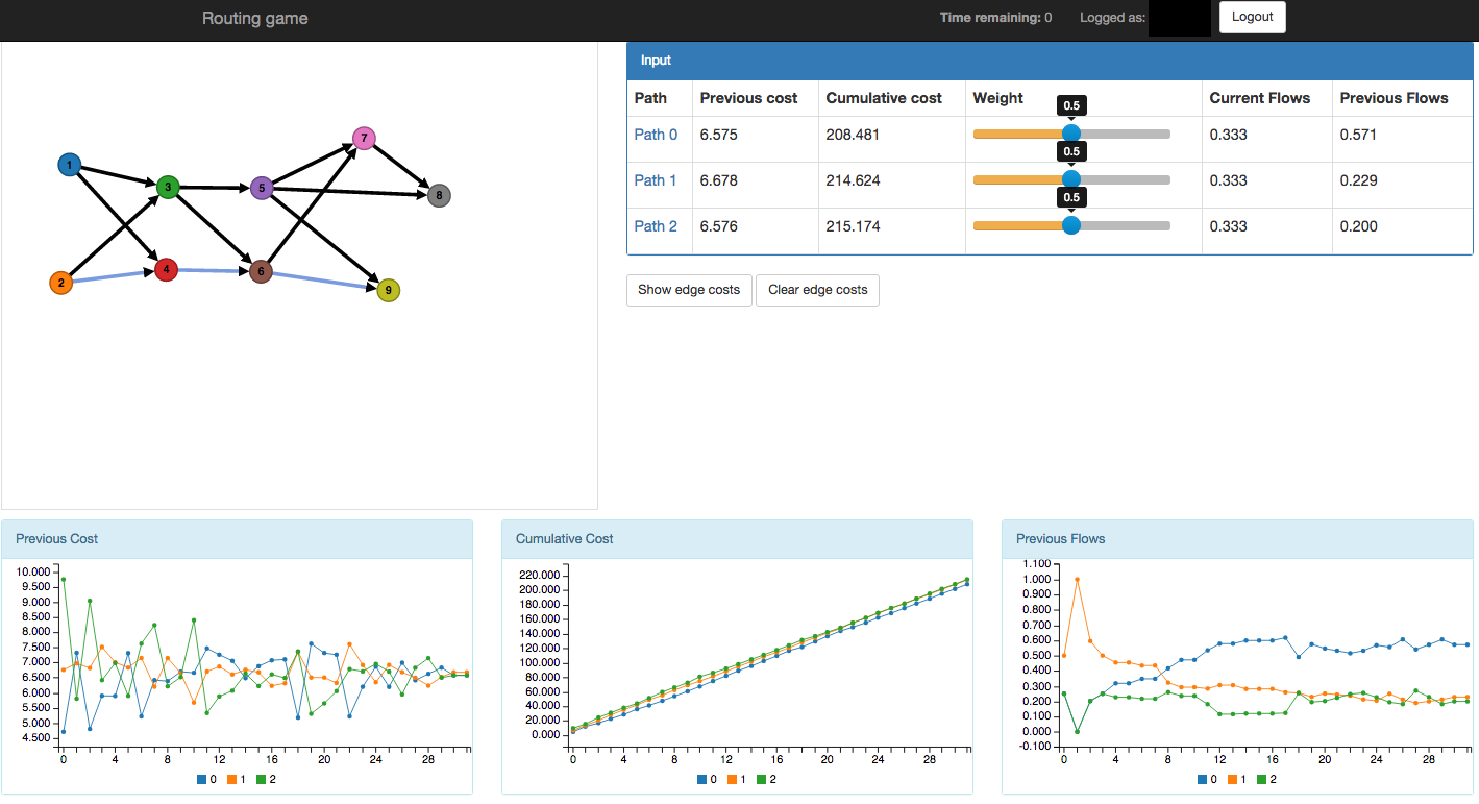
\includegraphics[width=.72\textwidth]{images/user_interface.pdf}\hspace{.03\textwidth}%
%\missingfigure[figwidth=.3\textwidth]{System block diagram}
\caption{\footnotesize Screenshot of the client side of the routing game application. The table is the main interface on the client side, and can be used by the player to set weights on the different paths, using the sliders. The weights determine the flow distribution $\bar x^{(t+1)}_k$. The table also show the previous flows ($x^{(t)}_k$), the previous costs $(\bar \ell^{(t)}_k)$, and the cumulative costs $\bar L^{(t)}_k = \sum_{\tau \leq t} \bar \ell^{(\tau)}_k$. Clicking a path will also highlight the path on the graph. The bottom charts show the full history of flows, costs, and cumulative losses.}
\label{fig:game_interface}  
  %\caption{Block diagram of the system. At iteration $t$, each player $p_k$ uses the cost vector history $(\bar \ell_{k}^{(t-1)}, \bar \ell_k^{(t-2)}, \dots)$ to make the routing decision vector $\bar x_k^{(t)}$. The server then computes the cumulative flow on each edge and returns the local cost vector history $(\bar \ell_{k}^{(t)}, \bar \ell_k^{(t-1)}, \dots)$ for player $p_k$, then the game proceeds to iteration $t+1$.}
\end{figure*}
%-----------------------------------------------------------------------------------------------------------------------------------------------------------------
%============================================================================================
\section{The Routing Game Web Application}
\label{sec:experiment}
\begin{figure}[h!]
  \centering
  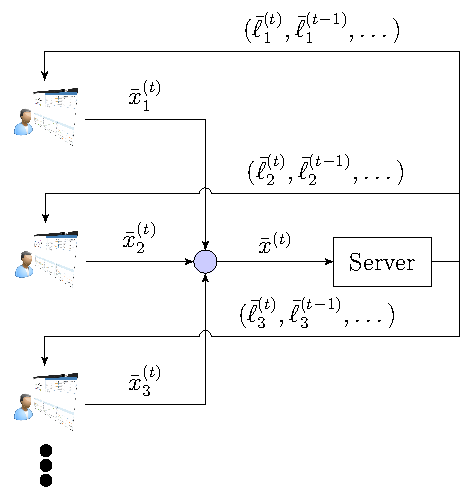
\includegraphics[width=.32\textwidth]{images/diagram.pdf}
  \caption{\footnotesize General architecture of the system. During iteration $t$, the clients input the current values of the distributions $\bar x^{(t)}_k$ and send them to the server. At the end of the iteration, the server uses these values to compute the cost functions $\bar \ell^{(t)}_k$ and sends them back to the clients.}
  \label{fig:system_block_diagram}
\end{figure}
%-----------------------------------------------------------------------------------------------------------------------------------------------------------------
% \begin{figure*}
%   \centering
%   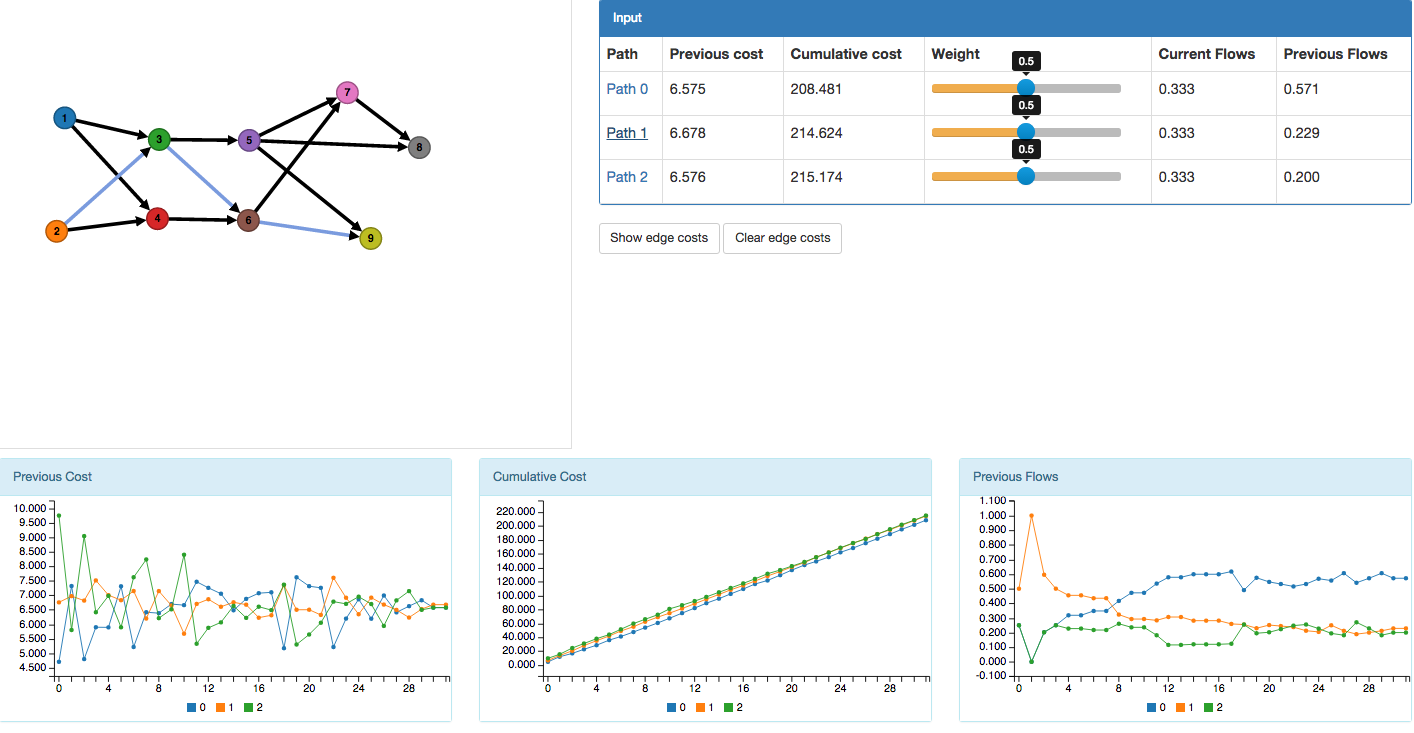
\includegraphics[width=160mm]{images/user_interface}
%   \caption{Web interface for the routing game.}
%   \label{fig:web_interface}
% \end{figure*}
%-----------------------------------------------------------------------------------------------------------------------------------------------------------------

We developed a web application that implements the repeated routing game described in Section~\ref{sec:model}. The general architecture of the system is summarized in Figure~\ref{fig:system_block_diagram}. It consists of a client interface that is used by human participants, shown in Figure~\ref{fig:game_interface}, and a backend server that is responsible for collecting inputs from the clients, updating the state of the game, then broadcasting current information to each player.



%
% \tikzstyle{block} = [draw, fill=white, rectangle,
% minimum height=3em, minimum width=6em]
%
% \tikzstyle{block} = [draw,fill=blue!20,minimum size=2em]
%
% \tikzstyle{sum} = [draw, fill=white, circle, node distance=1cm]
% \tikzstyle{input} = [coordinate]
% \tikzstyle{output} = [coordinate]
% \tikzstyle{pinstyle} = [pin edge={to-,thin,black}]

A root user can set up the game by creating a graph and defining the cost functions on each edge. Then once a game is set up, players can log in to the client interface, and each player is assigned an arbitrary origin node and destination node on the graph. Once the game starts, it is played in iterations, such that each iteration lasts a specified period of time shown by the timer on top of the client interface (each iteration lasts $30$ seconds in our experiments). Each player $k$ can use the sliders to set her flow distribution $x^{(t)}_k$ during iteration $t$. At the end of the iteration, the server uses the values of $x_k^{(t)}$ for all players $k \in \{1, \dots, K\}$ to compute the cost functions $\ell^{(t)}_k$, then sends this information to the client side, which then updates the charts and the table with the last value of the cost. Note that client $k$ only has access to the information about player $k$, so in this sense, the learning is completely distributed, as players do not observe the decision or the costs of other players. The decisions of the players $(\bar x_k^{(t)})$ and the costs $(\bar \ell^{(t)}_k)$ are logged by the server, with no additional identifiable information about the players.

The code for the web application is available on Github at the following url: \texttt{github.com/kietdlam/routing}. To illustrate the methods proposed in this article, we ran the experiment on a small network (shown in the interface in Figure~\ref{fig:game_interface}), with $5$ players. The numerical results are discussed in the next section.



%We simulate the proposed methods with a routing game system that implements the behavior of the network. The system is implemented with a web framework that is accessible to players through their browser. Players are assigned a unique origin and destination node pair and are tasked to assign a flow distribution to the paths between this pair at each turn of the game. The game calculates the cost along each edge of the network after all players have submitted their flow distribution for the turn. Each player then receives feedback with the local information of the cost for each path. The players then use this path cost history to assign a new flow distribution at the subsequent turns with the objective of minimizing their cumulative path cost.


% \begin{figure}
%   \centering
%   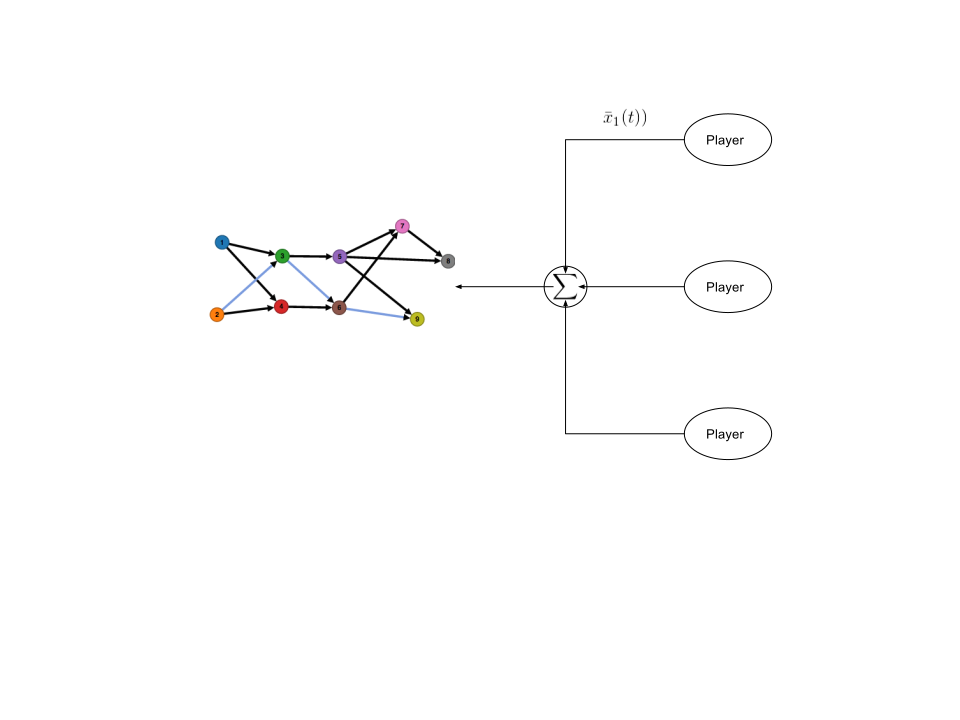
\includegraphics[width=0.5\textwidth]{images/game_system}
%   \caption{Player normalized cost.}
%   \label{fig:normalized_costs}
% \end{figure}

%To address a player who may be at a disadvantage due to having longer paths or more congested paths because of the topology of the network, we normalized the cumulative path cost of each player with their cumulative path cost at equilibrium calculated with Algorithm~\ref{alg:MD}.


%============================================================================================
%============================================================================================

%-----------------------------------------------------------------------------------------------------------------------------------------------------------------
\begin{figure*}
  \centering
  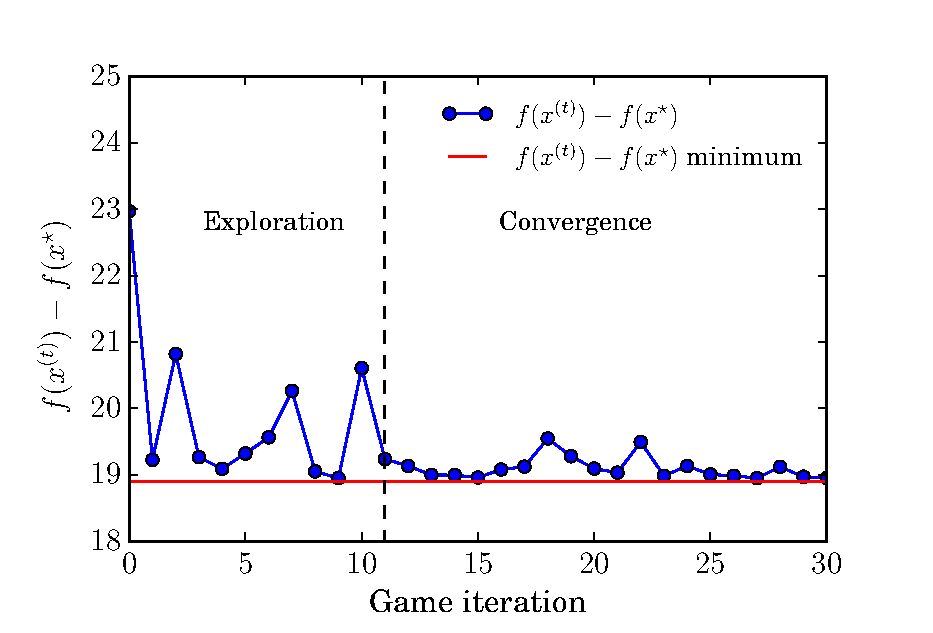
\includegraphics[width=0.33\textwidth]{images/global_potential_function.eps}%
  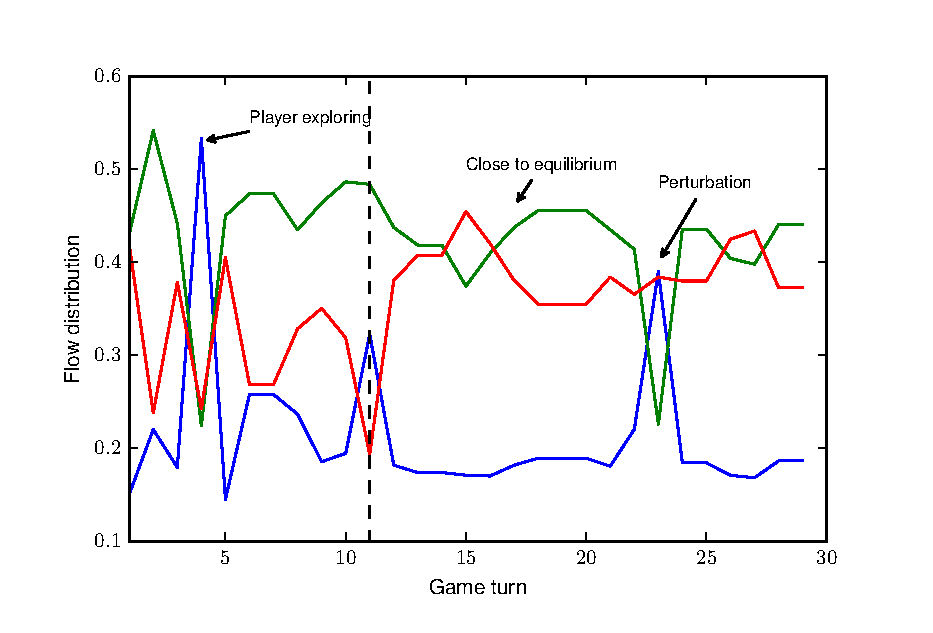
\includegraphics[width=0.33\textwidth]{images/player_behavior.eps}%
  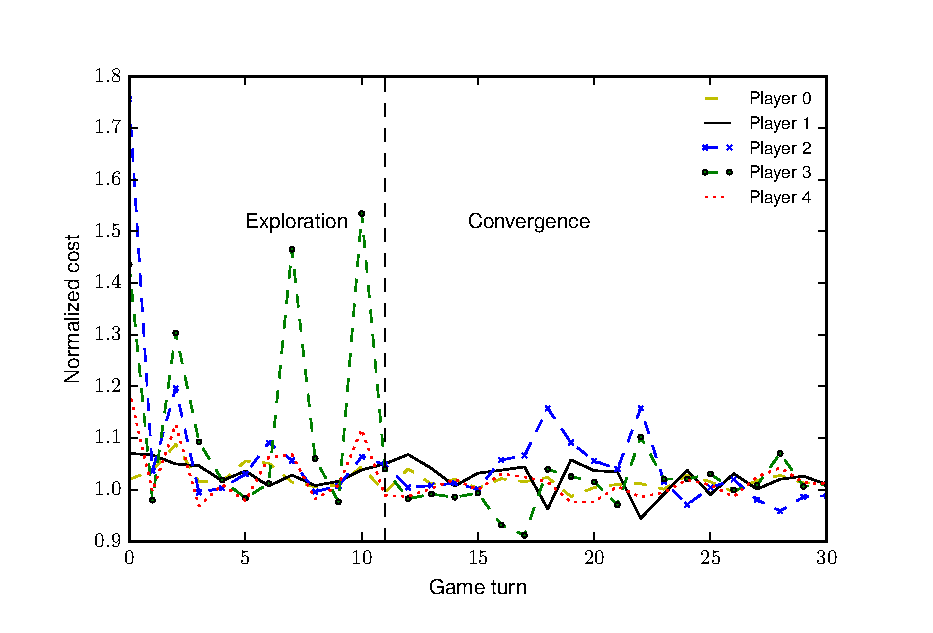
\includegraphics[width=0.33\textwidth]{images/players_costs.eps}%
  \caption{\footnotesize Exploration and convergence to equilibrium. The left figure shows the distance to equilibrium, measured by the Rosenthal potential $f(x^{(t)}) - f(x^\star)$ as a function of iteration $t$, where $x^{(t)} = (x_1^{(t)}, \dots, x_K^{(t)})$ is the joint decision of all players. The middle figure shows the flow distribution for a given player, and the right plot shows the costs of all players, normalized by the equilibrium costs (so that their values are comparable).}
  \label{fig:global_potential}
\end{figure*}
%-----------------------------------------------------------------------------------------------------------------------------------------------------------------

\section{Experimental Results}
\label{sec:results}
We use the data set collected by the experiment to illustrate the estimation and prediction problems proposed in Section~\ref{sec:estimation}, and give some comments on the decision dynamics of the players.
%-----------------------------------------------------------------------------------------------------------------------------------------------------------------
\subsection{Distance to equilibrium}
First, we evaluate whether the (distributed) decisions of the players converges to the Nash equilibrium of the game. The distance to equilibrium can be measured simply by the Rosenthal potential defined in Proposition~\ref{prop:potential}. Figure~\ref{fig:global_potential} shows the potential $f(x^{(t)}) - f(x^\star)$ as a function of iteration $t$, as well as the corresponding player costs $\braket{\ell^{(t)}_k}{x^{(t)}_k}$ of the players. We can observe that at the beginning of the game, there is a clear exploration phase in which players tend to make aggressive adjustments in their distributions, while during later turns, the adjustments become less aggressive and the joint distribution $x^{(t)}$ remains close to equilibrium (as measured by the potential function $f$). The system does move away from equilibrium at some later turns (due to a player performing an aggressive update, see for example turn $22$ in Figure~\ref{fig:global_potential}), but it quickly recovers in general.

%We can describe the convergence of the system more concretely by evaluating the Rosenthal potential of the game at each turn from Proposition~\ref{prop:potential}. From Figure~\ref{fig:global_potential}, the potential of the system oscillates rapdily in the exploration phase and then converges to the minimal potential. The system also shows robustness seen in Figure~\ref{fig:global_potential} where it recovers from perturbations in the convergence phase.

% This consolidation from the players can be seen by Figure~\ref{fig:global_potential}, where the player makes aggressive assignments in reaction to observing their cost, then converges to a flow distribution. The player perturbs the system near the end, but quickly reverts to the optimal flow distribution.

%\begin{figure}[h]
%  \centering
%  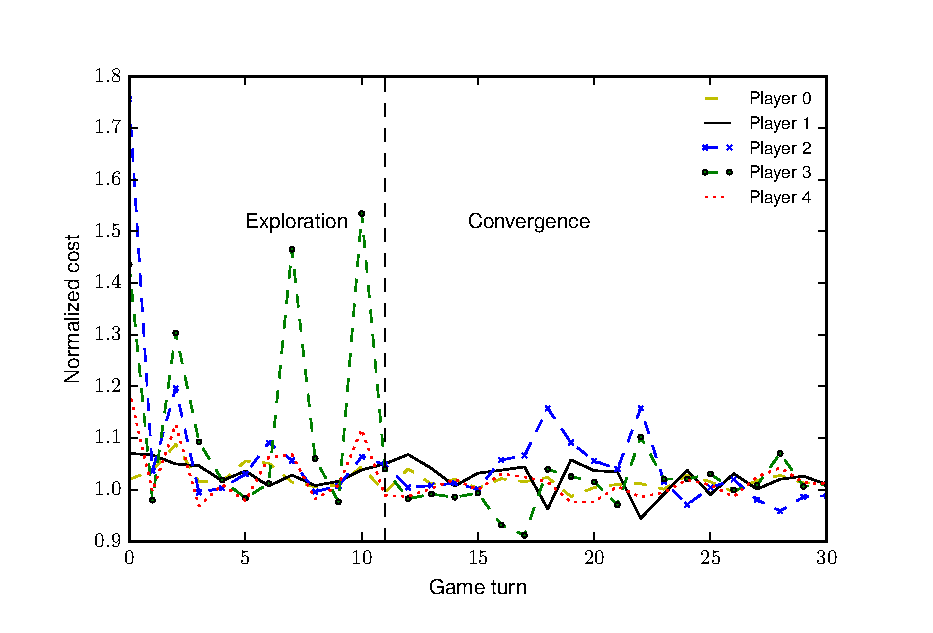
\includegraphics[width=0.5\textwidth]{images/players_costs}
%  \caption{Player cost normalized by equilibrium cost.}
%  \label{fig:normalized_costs}
%\end{figure}
%
%\begin{figure}
%  \centering
%  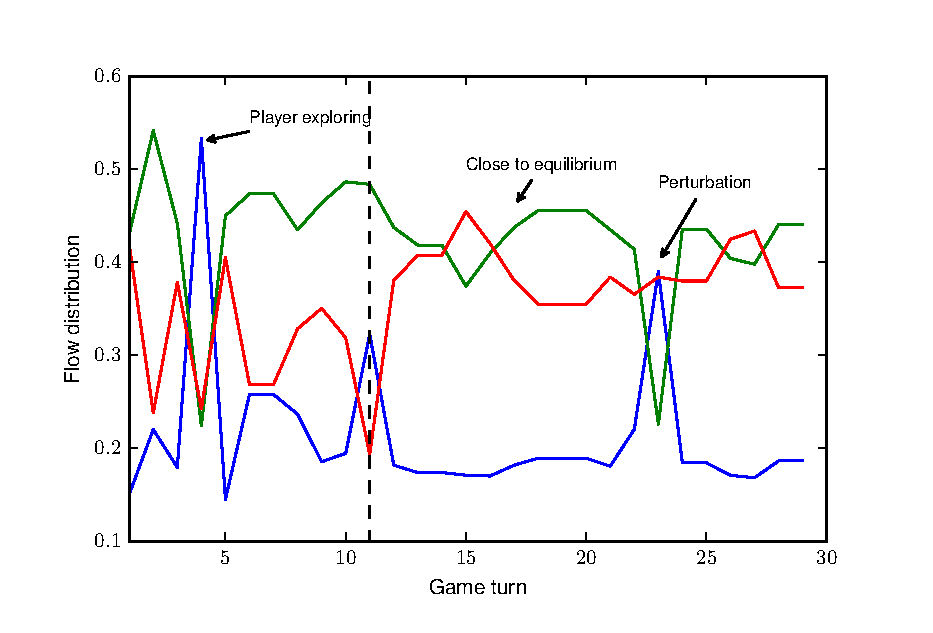
\includegraphics[width=0.5\textwidth]{images/player_behavior}
%  \caption{A player flow distribution assignment for the game.}
%  \label{fig:player_behavior}
%\end{figure}


\begin{figure}[h!]
\centering
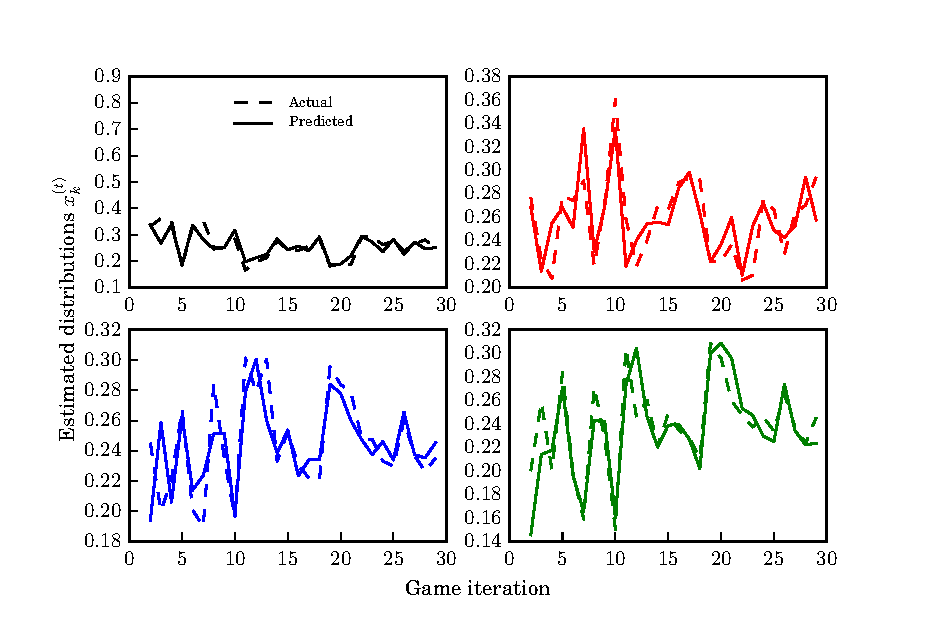
\includegraphics[width=.47\textwidth]{images/estimated_distribution.eps}
\caption{Comparison of the distributions $x^{(t)}_k$ of the estimated model to the actual distributions $\bar x^{(t)}_k$, for player $k = 2$. Each subplot corresponds to a path.}
\label{fig:estimated_distributions}
\end{figure}
%-----------------------------------------------------------------------------------------------------------------------------------------------------------------
\subsection{Estimation and prediction}
We now apply the method proposed in Section~\ref{sec:estimation} to estimate the learning rates of each player, then use the estimated rates to predict the decision of the players over a short horizon. In this section, we take the Bregman divergence to be the regularized entropy defined in Section~\ref{subsec:reg_entropy}, with $\epsilon = 10^{-3}$.

First, we solve Problem~\eqref{eq:estimation_eta} to estimate the learning rate sequence one term at a time. Figure~\ref{fig:estimated_distributions} compares the estimated distributions by the model, to the actual distributions. This shows that choosing one value of $\eta^{(t)}_k$ per turn makes it possible to closely fit the observations.

Then, we use the parameterized form $\eta^{(t)}_k = \eta_k^{(0)} t^{-\alpha_k}$, and estimate $\eta_k^{(0)}$ and $\alpha_k^{(0)}$ by solving the problem~\ref{eq:estimation_alpha_eta0}. The results of both methods are shown in Figure~\eqref{fig:moving_average_learning_rate}
When we estimate one term at a time, the resulting sequences have very large variations, and to better visualize them, we plot a moving average (over a window of $5$ iterations).

It was interesting and perhaps surprising to observe that when estimating learning rates one term at a time, in some rare instances, the objective $d^{(t)}_k(\eta_k^{(t)})$ is minimal at a negative $\eta_k^{(t)}$, which means that the player shifted the probability mass towards paths with \emph{higher} costs. One such example is given in the table below.
%-----------------------------------------------------------------------------------------------------------------------------------------------------------------
\begin{table}[h]
\centering
\small
\begin{tabular}{|c|c|c|c|}
\hline
Path & $\bar x^{(t)}$ & $\bar \ell^{(t)}$ & $\bar x^{(t+1)}$ \\
\hline
$p_1$ & $.198$ & $6.455$ & $.213$ \\
\hline
$p_2$ & $.218$ & $6.037$ & $.240$ \\
\hline
$p_3$ & $.280$ & $5.933$ & $.301$ \\
\hline
$p_4$ & $.304$ & $6.055$ & $.246$ \\
\hline
\end{tabular}
\caption{\footnotesize Example of an irrational behavior (corresponding to iteration $t = 12$ for player P2) which is hard to predict by the model. The inner product $\braket{\bar \ell_k^{(t)}}{\bar x^{(t+1)}_k - \bar x^{(t)}_k} > 0$, which means that the player shifts probability mass to paths with higher costs (in particular, the flow on path $p_1$ increased even though this is the worst path).}
\end{table}

%-----------------------------------------------------------------------------------------------------------------------------------------------------------------
\begin{figure}[h!]
  \centering
  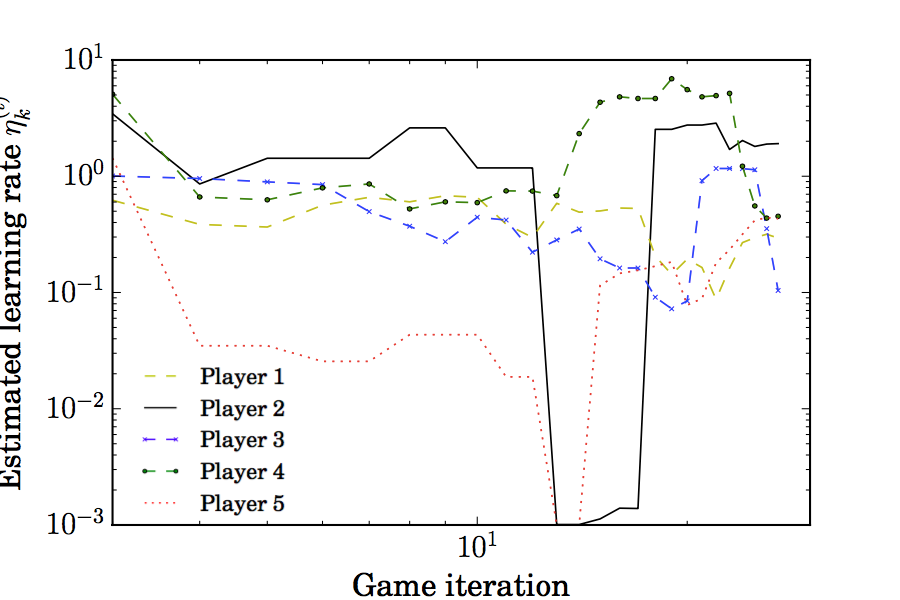
\includegraphics[width=0.37\textwidth]{images/moving_average_learning_rate}
  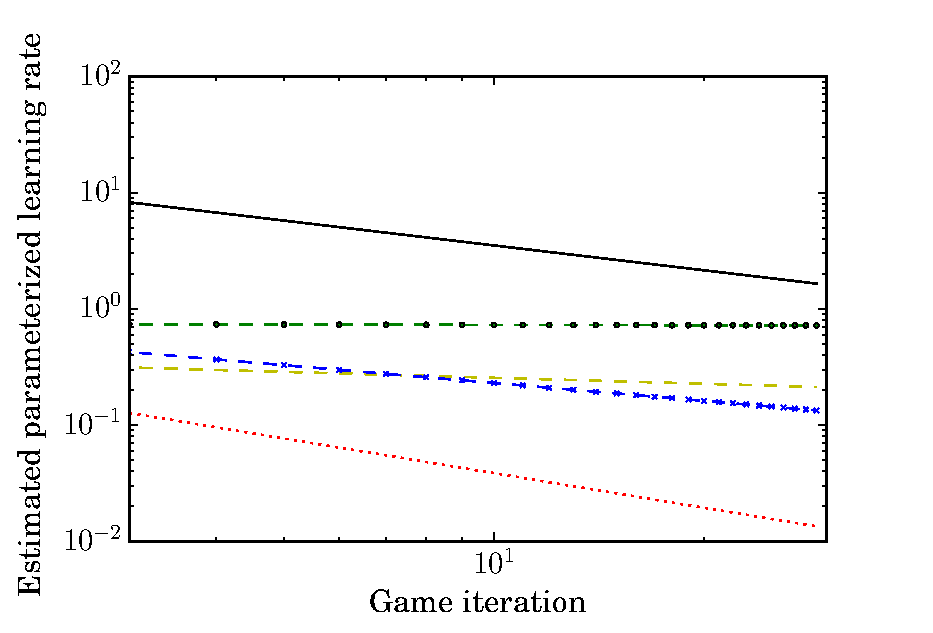
\includegraphics[width=0.37\textwidth]{images/sequence_rate}
  \caption{\footnotesize Estimated sequences of learning rates in logarithmic scale. In the top figure, we estimate one term of the sequence at a time then plot a moving average with a window length equal to $5$. In the bottom figure, we estimate for each player the initial term $\eta^{(0)}_k$ and the decay rate $\alpha_k$.\vspace{-.1in}}
  \label{fig:moving_average_learning_rate}
  \label{fig:sequence_rate}
\end{figure}
%-----------------------------------------------------------------------------------------------------------------------------------------------------------------





Next, we use the estimated learning rates to predict the distributions of the players over a short horizon $h \in \{1, \dots, 8\}$. More precisely, given a horizon $h$, we compute, at each iteration $t$, the estimated learning rates up to $t$, then propagate the model forward from $t$ to $t+h$, by iteratively applying the function $g$ defined in~\eqref{eq:propagation}.

We evaluate each method by computing the average Bregman divergence (per player and per iteration) between the predicted distribution $x^{(t+h)}_k$ and the actual distribution $\bar x^{(t+h)}_k$,
\[
\frac{1}{K} \sum_{k = 1}^K \frac{1}{t_{\max} - t_{\min}} \sum_{t = t_{\min}}^{t_{\max}-1} D_{\psi_k} (\bar x^{(t+h)}_h, x^{(t+h)}_k),
\]
where $t_{\min}$ is taken to be equal to $5$ (so that there is always a minimal history of observations to estimate the parameters). The results are given in Figure~\ref{fig:predictions_divergence}. One can observe that for all methods, as the horizon $h$ increases, the average divergence increases, since the modeling errors propagate and the quality of our predictions degrade. The best overall performance is obtained with the parameterized model $\eta^{(t)}_k = \eta^{(0)}_k t^{-\alpha_k}$, although for $h = 1$, the best prediction is achieved using the per-iteration estimate of $\eta^{(t)}_k$. 

\begin{figure}[h!]
  \centering
  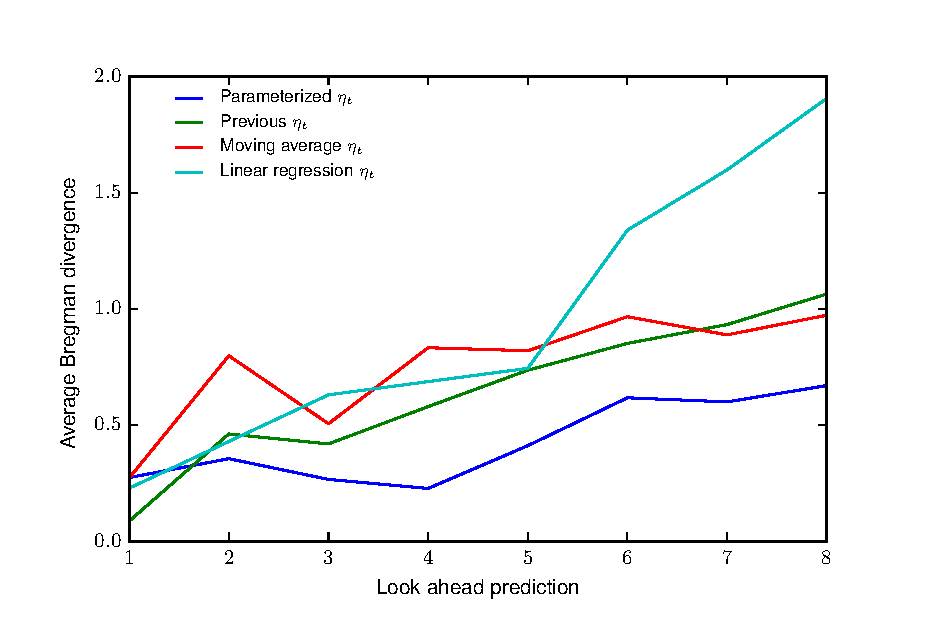
\includegraphics[width=0.37\textwidth]{images/predictions_divergence}
  \caption{\footnotesize Average Bregman divergence per player and per iteration, between the predicted distributions and the actual distributions, as a function of the prediction horizon.\vspace{-.1in}}
  \label{fig:predictions_divergence}
\end{figure}

%\begin{figure}[h]
%  \centering
%  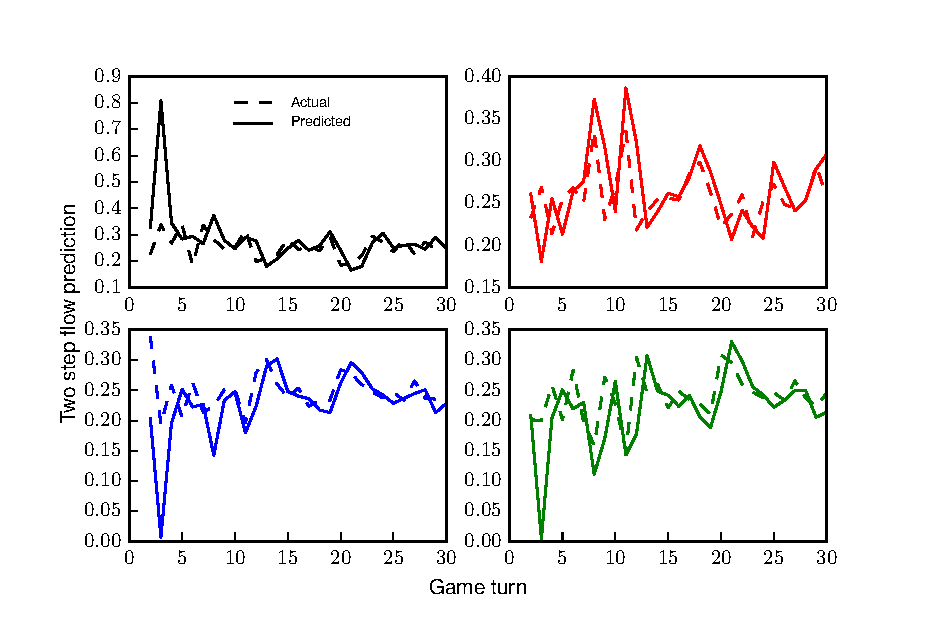
\includegraphics[width=0.5\textwidth]{images/two_steps_predictions}
%  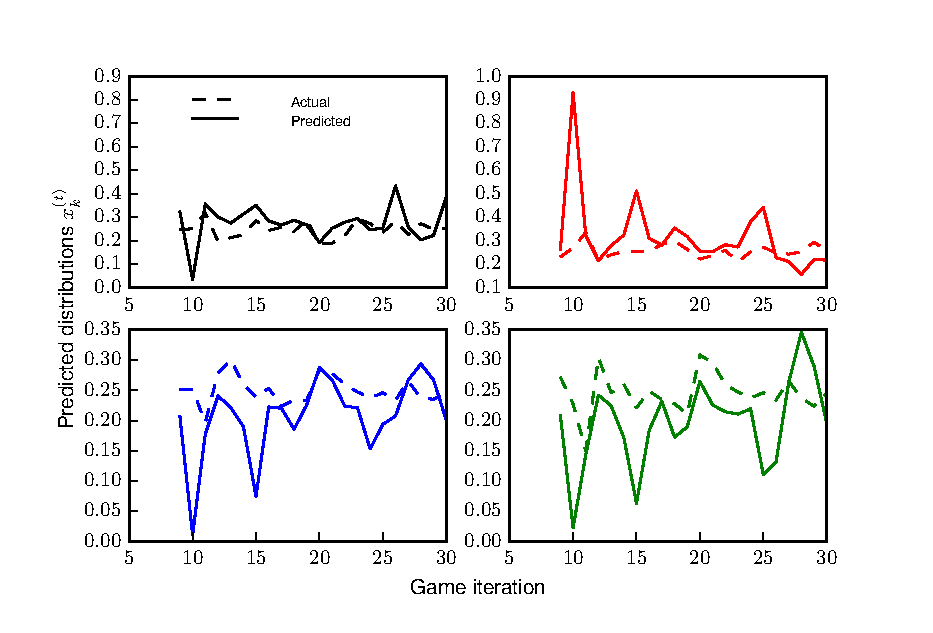
\includegraphics[width=0.5\textwidth]{images/eight_steps_predictions}
%  \caption{\footnotesize Comparison of predicted distribution (solid lines) and actual distribution (dashed lines) for a given player $k$. The prediction horizon for the top figure is $h = 2$, and for the bottom figure $h = 8$. Each subplot corresponds to a different path $p \in \Pcal_k$.}
%  \label{fig:parameterized}
%\end{figure}

%-----------------------------------------------------------------------------------------------------------------------------------------------------------------

%============================================================================================
\section{Conclusion}
\label{sec:conclusion}
We proposed a problem of model estimation in the routing game, to fit a distributed learning model to sequential observations of player decisions. The estimated model can then be used to predict the decisions at future iterations, or, more generally, as a plant model in an optimal control problem.

We considered in particular a model based on the mirror descent algorithm, parameterized by a DGF $\psi_k$ and a sequence of learning rates $(\eta^{(t)}_k)$, and gave an intuitive interpretation of how this model can describe player behavior. We showed that the problem of estimating one term of the learning rate sequence is convex in the case of the KL divergence (it remains open to prove this result for other Bregman divergences). To control the complexity of the model and to make the estimation consistent with the theoretical assumptions (decreasing learning rates), we proposed to parameterize the sequence with an initial term $\eta_k^{(0)}$ and a decay rate $\alpha_k \in (0, 1)$. When we tested these methods on data collected from our routing game interface, the parameterized sequence estimation outperformed the other methods on the prediction task. Our test results suggest that the mirror descent model can be a good descriptive model of player behavior, although in some rare cases, a player decision can be hard to model (e.g. when a player increase traffic assignment on previously bad routes).

This estimation problem can be extended in several ways: First, in our method, we fixed the DGF to be the negative entropy (regularized in order to avoid situations in which the estimation problem is ill-posed). One could also estimate the DGF itself, in addition to estimating the learning rates. One natural way to pose the estimation problem is to consider a finite collection of distance generating functions $\{\psi_i\}_{i \in \Ical}$, then to assume that each player $k$ uses a linear combination with weights $\theta_k$ $\psi = \sum_{i} \theta_{k, i} \psi_i$, then estimate the parameter vector $\theta_k$. 
\newpage
%============================================================================================
%
% The following two commands are all you need in the
% initial runs of your .tex file to
% produce the bibliography for the citations in your paper.
\bibliographystyle{abbrv}
\bibliography{bib}  % sigproc.bib is the name of the Bibliography in this case
% You must have a proper ".bib" file
%  and remember to run:
% latex bibtex latex latex
% to resolve all references
%
% ACM needs 'a single self-contained file'!
%
%APPENDICES are optional
%\balancecolumns
%============================================================================================

% That's all folks!
\end{document}

%%% Local Variables:
%%% mode: latex
%%% TeX-master: t
%%% End:
